%% Royal Society Interface - single-column manuscript
%% CRG-LLM: agents track the prompt, not the risk

\documentclass[openacc]{rsproca_new}

% packages (single column: no multicol)
\usepackage{amsmath}
\usepackage{booktabs}
\usepackage{multirow}
\usepackage{eurosym}
\usepackage{graphicx}
\graphicspath{{figures/}}

\jname{rsif}
\Journal{J R Soc Interface\ }

\begin{document}

\title{Large language model agents in a collective-risk social dilemma: cooperation tracks the prompt, not the risk}

\author{Anonymous author(s)}

\address{Anonymous affiliation}

\subject{artificial intelligence, behaviour, evolutionary game theory}

\keywords{large language models, collective-risk social dilemma, cooperation, risk sensitivity, prompt salience, group composition, multi-agent systems}

\begin{abstract}
Collective-risk social dilemmas, of which climate change is the archetype, reward a group only if its pooled contribution crosses a threshold before a probabilistic catastrophe. In the canonical human experiment, cooperation rises steeply with the stated risk. As large language models (LLMs) are increasingly deployed as autonomous agents and as surrogates for human decision-makers, we ask whether they reproduce this risk sensitivity. We ran eight instruction-tuned models -- seven open-weight models spanning three families and 7--72 billion parameters, plus a frontier API model -- as six-agent groups in a replication of the collective-risk dilemma, crossing catastrophe risk ($p=0.1,0.5,0.9$) with language (English, Vietnamese) and, in a second study, with the prosocial composition of the group. No model reproduced the human pattern. Because target-reach is at ceiling in most conditions, and a ceiling cannot express a risk response, we report the decisive test: in the subset of conditions where reach is genuinely uncertain -- neither ceiling nor floor, exactly where a risk-responsive agent has most to gain -- a ninefold increase in catastrophe risk moves contributions by $+0.97$ of a possible $240$ ($95\%$ CI $[-2.2,+4.1]$, $P=0.54$) in the open-weight panel and $+7.5$ ($95\%$ CI $[-6.3,+21.2]$, $P=0.26$) in the frontier model. Set against this null, three manipulations delivered through the prompt rather than through the incentive structure each move the same quantity by one to two orders of magnitude more: printing the running pool total (up to $95.3$ points), changing the prosocial composition of the group ($31.8$--$112.4$ points), and switching the language from English to Vietnamese ($146.8$ points, flipping the frontier model from a $100\%$ to a $0\%$ reach rate). Group composition acts through a strikingly simple mechanism: contributions fall almost perfectly linearly in the number of selfish-persona agents ($R^2$ up to $0.95$), so whether a group succeeds is decided by where that line crosses a fixed threshold, not by the risk of failing to cross it. In-situ comprehension probes locate the boundary of what the agents can do: they recite the rules ($93.8$--$100\%$) and read printed values near-perfectly, while summing the pool across rounds fails in small models and recovers with scale ($14\%$ to $88\%$). We stress a limitation that bounds all such studies, ours included: our prompt names the equal-split solution, and several models lock onto exactly it. We argue that behavioural claims about LLM agents must be tested against prompt-side controls before they are attributed to preferences.
\end{abstract}

\begin{fmtext}
The prevention of dangerous climate change is a collective-risk social dilemma: many actors must jointly invest enough to keep a shared catastrophe from occurring, yet each actor is individually tempted to free-ride on the investment of others~\cite{milinski2008collective,hardin1968tragedy,dawes1980social}. In laboratory social dilemmas, humans sustain cooperation through reciprocity and costly punishment and respond to the material stakes at hand~\cite{fehr2002altruistic}. Laboratory versions of this dilemma have a sharp empirical signature. When Milinski and colleagues had groups of six people play a ten-round threshold game in which failing to reach the target triggered the probabilistic loss of everything they had kept, the fraction of groups that reached the target rose steeply with the announced risk of loss - from essentially zero when the risk was low to about half when the risk was high~\cite{milinski2008collective}. Humans, in other words, cooperate more when more is at stake.
\end{fmtext}

\maketitle

\section{Introduction}

Large language models (LLMs) are now used both as autonomous agents that negotiate, plan and transact on a user's behalf, and as inexpensive surrogates for human participants in the social and economic sciences~\cite{horton2023large,argyle2023out,aher2023using}. A growing literature places these models inside classic games and finds that they can cooperate, reciprocate and punish, but often in ways that diverge from human play, and not always in the same direction: some models are strikingly prosocial and forgiving in repeated dilemmas~\cite{fontana2024nicer,phelps2023investigating}, whereas others retaliate unforgivingly after a single defection~\cite{akata2023playing} or fail to sustain a shared resource without institutional scaffolding~\cite{piatti2024cooperate}. If such agents are to be trusted in, or used to forecast, high-stakes collective decisions, we need to know how they behave when the dilemma is structured by \emph{risk} rather than by a fixed payoff matrix, because it is precisely the response to risk that gives the human collective-risk dilemma its policy relevance.

This question is entangled with a methodological one that recurs throughout the study of LLM behaviour. When a model deviates from the human pattern, the deviation admits two very different readings. It may be a genuine behavioural disposition - the model ``understands'' the situation and nonetheless chooses differently - or it may be an artefact of comprehension, in which the model has simply misread the rules, the history or the current state. These two readings have opposite implications for whether scaling, prompting or fine-tuning will change the behaviour, yet most behavioural studies of LLMs do not measure comprehension directly and therefore cannot distinguish them. Recent work on the prisoner's dilemma has begun to close this gap by interleaving behavioural play with a battery of understanding checks, asking the model to report the rules, the game history and the current state, and scoring the answers against ground truth~\cite{fontana2024nicer}.

A third problem is specific to reporting null results in threshold games, and it is the one that most limits what can be concluded from a study of this kind. When agents cooperate enough to clear the threshold in essentially every game, the outcome variable is censored at its ceiling: a risk response of the human size could not appear in it even if it existed. A flat reach rate is therefore weak evidence on its own. The remedy is to find conditions in which the outcome is genuinely uncertain and to test the risk response there, and a manipulation that varies how cooperative the group is provides exactly such conditions.

Here we bring these questions together for the collective-risk social dilemma. We instantiated the Milinski experiment with LLM agents, replacing each of the six human players with an instruction-tuned model, and swept the announced catastrophe risk across the same three levels used with humans. To ask whether behaviour is bounded by capability, we placed seven open-weight models spanning three families and an order of magnitude in size, from 7 to 72 billion parameters, in the identical protocol, and added a frontier API model to test whether the pattern is an artefact of open-weight models alone. To separate disposition from comprehension, we adapted the understanding-check methodology of Fontana et al.~\cite{fontana2024nicer} from the two-player prisoner's dilemma to the $N$-player threshold game, probing each model \emph{in situ} on the very prompts from which it was making decisions, with all answers graded against the game engine's ground truth. To break the ceiling and obtain uncensored conditions, we ran a second study that varied the prosocial composition of the group, assigning between zero and six of the six agents a selfish persona. Finally, because these models are deployed multilingually and the collective-risk framing has an intrinsic numerical structure, we ran every condition in both English and Vietnamese.

Four findings organise the paper. First, no model reproduces the human risk response, and the null is not an artefact of censoring: in the conditions where reach is genuinely uncertain, tripling the catastrophe risk moves contributions by an amount statistically indistinguishable from zero. Second, three manipulations that carry no incentive information whatsoever - printing the running pool total, changing who is in the group, and changing the language - each move contributions by one to two orders of magnitude more than risk does. Third, the composition effect has a simple and highly regular form: contributions fall linearly in the number of selfish agents, and success is decided by where that line crosses the fixed threshold, which explains why nominally similar models fail at completely different compositions. Fourth, comprehension probes bound what this can be attributed to: the agents recite the rules and read printed quantities near-perfectly, and the one genuine cognitive gap, summing the pool across rounds, is a small-model deficit that closes with scale. Throughout we are careful about a threat that applies to this literature generally and to our design in particular: our prompt names the equal-split solution, and some models reproduce it exactly, so cooperative-looking behaviour cannot be cleanly separated from compliance with a supplied focal point.

\section{Material and methods}

\subsection{The collective-risk social dilemma}
We reproduced the parameters of the canonical human experiment~\cite{milinski2008collective}. Six players each began with an endowment of \euro{}40. Over ten rounds, each player privately and simultaneously chose to contribute $0$, $2$ or $4$ to a common pool. If the pooled total reached the target of \euro{}120 by the end of the game, players kept whatever they had not contributed; if the target was missed, then with probability $p$ - the catastrophe risk - every player lost all remaining private money. The maximum achievable pool is $6\times4\times10=240$, so the target of $120$ can be met if players contribute, on average, half of the maximum. We used the three risk levels of the original study, $p\in\{0.1,0.5,0.9\}$. For humans, the fraction of groups reaching the target rose with risk, from $0\%$ at $p=0.1$ to $10\%$ at $p=0.5$ to $50\%$ at $p=0.9$~\cite{milinski2008collective}; this monotone increase is the behavioural benchmark against which we compare the models.

\subsection{Language-model agents and the game loop}
Each human player was replaced by an instruction-tuned LLM. We built a configuration-driven engine, in the style of agent-based game frameworks for LLMs~\cite{buscemi2025fairgame}, in which the six agents in a group were homogeneous (the same model) and, in the baseline study, anonymous (neutral identifiers, no assigned personas). On each round, every agent received a natural-language prompt containing the rules of the game and the complete round-by-round history, and was asked to end its reply with a line of the form \texttt{CONTRIBUTION:}~$c$ with $c\in\{0,2,4\}$, which we parsed deterministically. Agents therefore had full-history memory and a neutral framing that neither encouraged nor discouraged cooperation. One property of this prompt matters for every interpretation that follows and we state it plainly: in describing the target it also names the equal-split solution, telling the agent that \euro{}120 corresponds to ``an average of 2 per player per round'' and adding the worked example that contributing 2 every round leaves 20 at the end. The prompt therefore supplies a risk-independent focal action. It is faithful to the information a human subject could trivially compute, but it means that an agent contributing 2 may be solving the dilemma or may simply be following the number in front of it, and our design cannot separate the two. We return to this in \S\ref{sec:limits}. Catastrophes were resolved by a single end-of-game lottery. That lottery is the weakest part of the implementation. It draws one uniform variate per repetition, seeded from the repetition index alone, so the same draws are shared across every model, language and risk level: the study contains ten independent lottery outcomes in total, not one per game. All ten happen to fall below $0.5$ (mean $0.276$), so at $p=0.5$ and $p=0.9$ every game that missed the target was recorded as a catastrophe. Realised catastrophe rates are therefore an artefact of the draw schedule and we exclude them from all inference; they are reported only descriptively. Open-weight models were served locally with vLLM at a $4096$-token context and decoded at temperature $0.7$ with a $512$-token cap. Sampling was seeded per turn from the experiment seed, the repetition, the round and the agent index, so that runs are reproducible and independent across repetitions while using common random numbers across the risk and language conditions, isolating the manipulated factor. The structure of the decision prompt is summarised in figure~\ref{fig:pipeline}(a).

We studied seven open-weight models spanning three families and roughly an order of magnitude in size: Qwen2.5 at 7B, 32B and 72B~\cite{qwen2025qwen25}; Gemma-2 at 9B and 27B~\cite{gemma2024gemma2}; and Llama-3.1 at 8B and 70B~\cite{grattafiori2024llama3}. The two 70--72B models were served with activation-aware weight quantisation. Each model played the full factorial of three risk levels by two languages with ten independent repetitions, giving $60$ games per model. Contributions were parsed without failure for all seven models (parse-failure rate $0\%$), so every game contributed valid data.

\subsection{Group composition: the persona study}
\label{sec:personamethods}
The baseline groups are homogeneous and neutral, which leaves target-reach at its ceiling in almost every cell and therefore unable to express a risk response. To break that ceiling we ran a second study that varies how prosocial the group is. Each agent's prompt was prefixed with a single sentence naming a disposition, either \emph{selfish} (``You are a selfish player: you only care about maximising your own final amount of money'') or \emph{cooperative} (``You are a cooperative player: you want the whole group to reach the target and avoid the disaster''). We swept the number of selfish agents in the group from $0$ to $6$ in unit steps, giving seven compositions, and crossed this with the same three risk levels and two languages. Nothing else in the prompt changed; in particular the payoffs, the target and the stated catastrophe probability were identical across compositions, so composition carries no incentive information about the game itself. Persona-to-seat assignment was permuted deterministically from the condition and repetition indices. This scheme is not a uniform random assignment - it yields only four to nine distinct seat patterns per mixed composition, and across the mixed compositions the six seats are not occupied by a selfish agent equally often ($\chi^2=23.0$ on $5$ d.f., $P=0.0003$; two seats are never selfish when exactly one agent is) - so we make no claims about seat position. We verified that this does not disturb the composition effect: adding the full seat arrangement to a model that already contains the number of selfish agents raises $R^2$ by only $0.005$--$0.029$, against the $0.48$--$0.75$ explained by the number alone. The composition study was run for the three smallest open-weight models (Qwen2.5-7B, Llama-3.1-8B, Gemma-2-9B) at ten repetitions, giving $1{,}260$ games, and for the frontier model at five repetitions, giving $210$ games.

\subsection{A frontier model arm}
\label{sec:frontiermethods}
All seven open-weight models share broad architectural and training conventions, so a pattern common to all of them might reflect that shared lineage rather than instruction-tuned LLMs generally. We therefore repeated both studies with a frontier API model, GPT-5.4-nano, accessed through its provider's chat completions interface at the provider's default temperature. Because API calls are metered we used five repetitions rather than ten, giving $30$ baseline games and $210$ composition games. This arm is a generalisation test, not a like-for-like comparison: the model is served by a third party, its decoding parameters are not under our control, and per-turn sampling seeds are not honoured by the interface, so its games are not paired with the open-weight games by common random numbers and are analysed separately throughout. It carries no comprehension probes.

\subsection{In-situ comprehension probes}
To test whether behaviour was bounded by understanding, we adapted the meta-prompting battery of Fontana et al.~\cite{fontana2024nicer} from the two-player prisoner's dilemma to the $N$-player collective-risk game. Twenty questions were organised along three axes: \emph{Rules} (the fixed structure of the game - available actions, endowment, target, number of rounds and, critically, the catastrophe probability), \emph{Time} (reading specific past events from the history) and \emph{State} (the current cumulative situation, including the running pool total). Every question had a closed-form ground truth computed by the game engine, so grading involved no second model. Probes were issued on the identical prompts from which the agent was deciding and were appended after the decision, so a probe cannot influence the decision it accompanies. The comprehension runs were nevertheless a separate execution of the game, using greedy decoding for a deterministic benchmark, and their behavioural trajectories therefore differ from those of the main behavioural runs; the two studies characterise the same agents and the same prompts, not the same game trajectories. Because the shared pool total is the quantity most likely to expose a difference between reading and computing, we ran a controlled A/B manipulation in which the running total was either hidden (the default) or printed in the prompt. This manipulation adds no information about incentives - the total is a deterministic function of a history the agent already has - so it serves as a salience control for the behavioural study as well as a comprehension probe, and we analyse its behavioural arm in \S\ref{sec:salience}. It was run for the five models in the comprehension panel at 7--32B. Probes used greedy decoding for a deterministic benchmark and yielded approximately $54{,}500$ graded probes per model. The comprehension panel used the same models as the behavioural study except that the 70B Llama was the Llama-3.3 revision rather than Llama-3.1; we keep the labels distinct throughout. Unparseable answers were graded as incorrect; the probe parse-failure rate was below $0.01\%$ for six of the seven models and $1.03\%$ for Llama-3.1-8B, where it was almost entirely confined to Vietnamese ($2.05\%$ of that model's Vietnamese probes). Accuracies are reported with Wilson $95\%$ confidence intervals~\cite{wilson1927}. These treat probes as independent, which they are not: probes are clustered within games, rounds and questions, so the intervals we plot are anti-conservative and should be read as a lower bound on uncertainty. Because the comprehension differences we rely on span tens of percentage points, this does not affect any conclusion drawn here, but it would matter for finer comparisons.

\subsection{Analysis and dependent variables}
Our primary behavioural dependent variables were the target-reach rate (the fraction of games in which the pool met \euro{}120) and the group contribution (the pooled total, out of $240$). We treated the realised catastrophe rate as secondary, because a single end-of-game lottery per game, with the draw shared across languages by the common-random-number scheme, yields only about ten effective draws per model and risk level and is therefore noisy. Contributions in the open-weight panel are analysed paired, because the design reuses sampling seeds across the risk and language conditions; the resulting within-pair correlations range from $0.32$ to $0.95$, so an unpaired analysis would discard real precision. Because reach is censored in most cells, we defined a subset of \emph{uncensored} cells - those model-by-composition-by-language cells in which the reach rate is strictly between $0$ and $1$, so that the outcome is genuinely in doubt - and report the risk response within them as the study's decisive test (\S\ref{sec:knifeedge}). This criterion is a function of the outcome variable, so we report it alongside three checks that are not: selection on a disjoint risk level, selection on a pre-outcome criterion derived from the fitted composition line, and an unselected regression of contribution on risk, composition and their interaction over all composition games. We also report the minimum effect the design could have detected. For the comprehension study the dependent variable was answer accuracy against the engine ground truth. All quantities were recomputed directly from the raw per-game and per-probe logs.

\begin{figure*}[t]
\centering
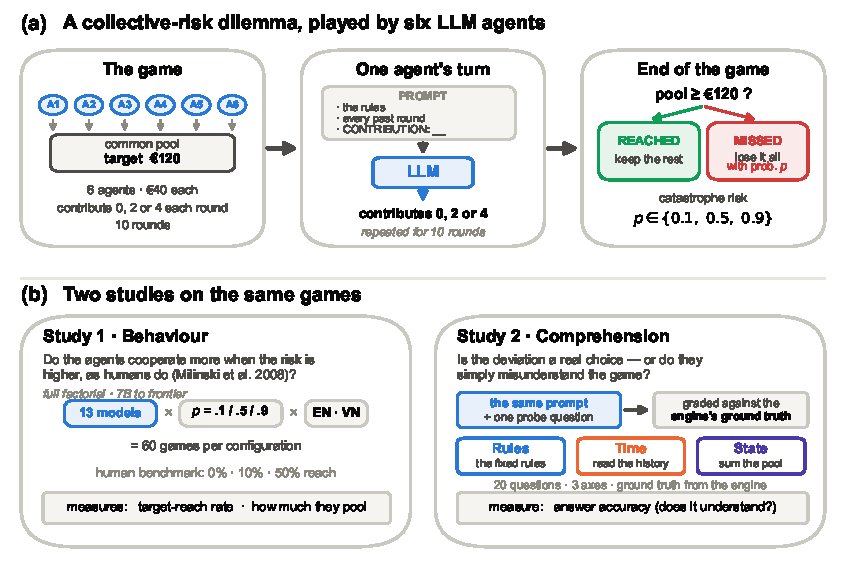
\includegraphics[width=\textwidth]{fig1_pipeline.pdf}
\caption{\textbf{Study design.} (a)~Six LLM agents play a faithful replication of the Milinski collective-risk dilemma: each of six agents starts with \euro{}40 and, over ten rounds, privately contributes $0$, $2$ or $4$ to a common pool from a prompt containing the rules and the full history; at the end, if the pool has not reached \euro{}120 the group suffers a catastrophe with probability $p\in\{0.1,0.5,0.9\}$. (b)~The same games feed two studies. Study~1 (behaviour) crosses seven models ($7$--$72$B) with three risk levels and two languages ($60$ games/model) and measures the target-reach rate and how much the agents pool. Study~2 (comprehension) appends a graded question to the identical prompt, scoring twenty questions along three axes (Rules, Time, State) against the engine's ground truth, to ask whether any deviation is a genuine choice or a misunderstanding.}
\label{fig:pipeline}
\end{figure*}

\section{Results}

\subsection{No model reproduces the human risk response}
Humans in the collective-risk dilemma cooperate more when the catastrophe is more likely; the models did not. Every model reached the target at the same rate at every risk level (figure~\ref{fig:risk}(a)), against a human benchmark that climbs from $0\%$ to $50\%$ across the same range. Six of the seven open-weight models reached the target in essentially every game regardless of risk (Qwen2.5-7B, Llama-3.1-8B, Gemma-2-9B, Gemma-2-27B and Qwen2.5-72B at $100\%$; Qwen2.5-32B at $96.7\%$), and the seventh, Llama-3.1-70B, reached it in exactly half of its games at each of $p=0.1$, $0.5$ and $0.9$.

This flatness is easy to describe and hard to test, and we are explicit about the limitation. Five of the seven models reached the target in all sixty of their games, so their reach rate has no variance and admits no regression on risk at all; a sixth varies only between $95\%$ and $100\%$. Reach is thus censored at the ceiling for six of seven models, and a positive risk response of the human size would be arithmetically undetectable in it. We therefore treat reach as descriptive and take group contribution, which is free to move in either direction, as the informative dependent variable.

Analysed paired, risk does move contributions. Every one of the seven models has a positive risk slope, and a paired $t$-test on the difference between $p=0.9$ and $p=0.1$ is significant for three of them: Gemma-2-9B ($+8.8$ points, $P=0.0023$), Qwen2.5-72B ($+3.2$, $P=0.0062$) and Gemma-2-27B ($+1.9$, $P=0.048$); the first two survive Bonferroni correction across the seven models. The response is real. What it is not is consequential. The largest effect any model shows across the entire risk range is $8.8$ of a possible $240$ - about one extra contribution of 2 from one agent in four of the sixty games - and it changes no outcome, since Gemma-2-9B already reached the target in every game at every risk level. Against the human benchmark, where the identical manipulation moves the fraction of successful groups from none to half, this is a response in the right direction and of the wrong order of magnitude.

One caveat about that effect deserves the same treatment we give Llama-3.1-70B below. Gemma-2-9B's response is entirely Vietnamese: in English it contributed exactly $120.0$ in all thirty games, a hard constant with no variance and no slope to estimate, while in Vietnamese it rose from $127.8$ to $145.4$ (slope $+22.0$, $P=0.0042$). Two of the fourteen model-by-language cells are constants of this kind, and Qwen2.5-7B sits at the $240$ ceiling in $16$ of its $60$ games. Both dependent variables are censored somewhere in this panel, and no analysis can recover a risk response from a cell with no variance.

\begin{figure*}[t]
\centering
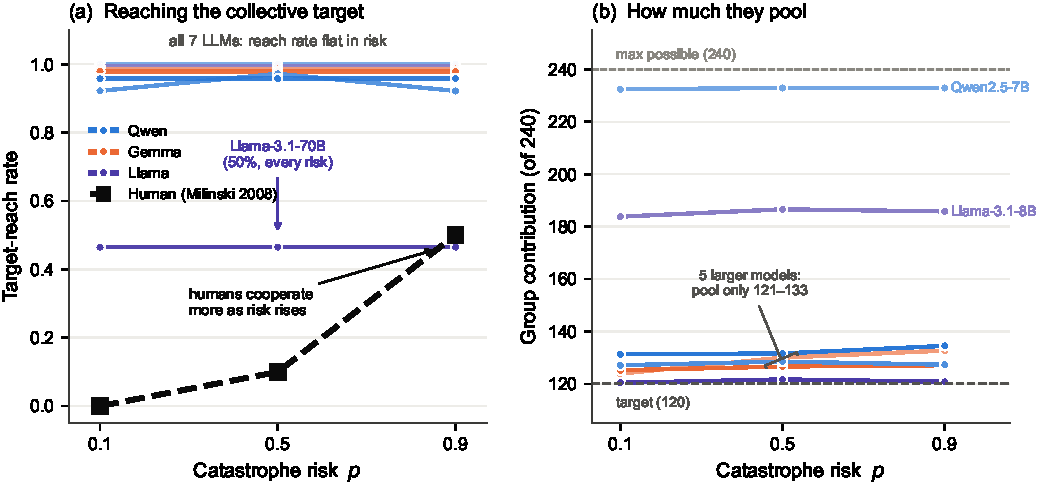
\includegraphics[width=\textwidth]{fig2_risk_insensitivity.pdf}
\caption{\textbf{No model reproduces the human risk response.} (a)~Target-reach rate against catastrophe risk for all seven open-weight models (colour denotes family; shade denotes size) and for humans (dashed). Every model's reach rate is flat in $p$; humans rise from $0\%$ to $50\%$. Llama-3.1-70B is flat at $50\%$. (b)~Group contribution (of a possible $240$) against risk. Contributions are essentially flat in $p$ (the one weak exception, Gemma-2-9B, is quantified in the text); the vertical spread reflects how economically each model plays, not risk sensitivity. In (a) five models sit exactly on $100\%$, so the curves are drawn with a small downward offset (at most $0.04$) purely so that all seven remain visible; no curve is drawn above its true value.}
\label{fig:risk}
\end{figure*}

\subsection{The null survives where the outcome is genuinely in doubt}
\label{sec:knifeedge}
The censoring objection is the strongest available defence of the models, and it deserves a direct test rather than a caveat. If reach sits at its ceiling, a risk response cannot appear in it; the flat curves of figure~\ref{fig:risk}(a) would then be uninformative about whether the agents are risk-sensitive. The composition study supplies the missing conditions. Varying the number of selfish agents moves groups off the ceiling and, in some cells, onto the knife edge, where roughly half of the games succeed and half fail. Those are the conditions in which a risk-responsive agent has most to gain from contributing more, and in which the outcome variable is free to move in either direction.

We therefore defined the uncensored cells as those with a reach rate strictly between $0$ and $1$, and tested the risk response inside them. Seven of the $42$ open-weight cells qualify and three of the $14$ frontier cells. The result is a clean null. Pooling the open-weight uncensored cells and pairing on the sampling seed, raising the catastrophe risk from $p=0.1$ to $p=0.9$ changes group contribution by $+0.97$ points of $240$ ($95\%$ CI $[-2.2,+4.1]$, $n=70$ pairs, $P=0.54$), and the reach rate by $+4.3$ percentage points ($0.514\to0.557$). In the frontier model the point estimate is larger but no more distinguishable from zero: $+7.5$ points ($95\%$ CI $[-6.3,+21.2]$, $n=15$ pairs, $P=0.26$), with reach moving $0.400\to0.467$. Not one of the ten individual uncensored cells shows a significant risk effect at $\alpha=0.05$, and four of the ten point in the wrong direction.

This null is not a failure of power. The paired differences in the open-weight uncensored set have a standard deviation of $13.1$ points, so with $70$ pairs the design detects an effect of $4.4$ points of $240$ with $80\%$ power; the observed estimate is $+0.97$ and its upper $95\%$ bound is $+4.05$. We can exclude, at conventional confidence, anything larger than a $4$-point response - against a human benchmark in which the same manipulation moves half of all groups across the threshold, a shift of $120$ points in the groups it moves.

Selecting cells on a function of the outcome variable is the obvious objection to this analysis, so we checked it three ways, none of which selects on the tested data. First, choosing the cells using only the $p=0.5$ games and testing on the disjoint $p=0.1$ and $p=0.9$ games returns the same estimate ($+0.97$, $P=0.54$). Second, selecting cells by a criterion computed before any outcome is observed - those whose composition places the fitted contribution line within $\pm30$ points of the threshold - widens the set to $13$ cells and $130$ pairs and gives $+1.34$ points ($95\%$ CI $[-0.7,+3.4]$, $P=0.19$). Third, abandoning selection entirely and fitting the risk-by-composition interaction to all $1{,}260$ open-weight composition games gives a risk coefficient of $+3.80$ per unit probability ($95\%$ CI $[-3.5,+11.2]$, $P=0.31$), implying $+3.0$ points across the full $p=0.1\to0.9$ sweep, with no significant interaction ($P=0.21$); the corresponding frontier estimate is $-0.07$ points ($P=0.99$). Every route to the question returns the same answer.

This is the decisive result of the risk analysis. In precisely the conditions where the ceiling argument does not apply - where the group is balanced on the threshold and the catastrophe is a live possibility rather than a formality - a ninefold change in the probability of losing everything moves behaviour by an amount indistinguishable from zero. The null is a property of the agents, not of the measurement.

\subsection{Scale buys economy, not risk sensitivity}
Although risk did not move the models, scale did move how much they cooperated. In every family the largest model pooled far less than the smallest, though the decline is not strictly monotonic (figure~\ref{fig:economy}). The smallest models over-contributed massively: Qwen2.5-7B pooled $232.7$ of a possible $240$, close to the ceiling, and Llama-3.1-8B pooled $185.4$. Every larger model converged toward the minimum that clears the threshold, pooling between $121$ and $133$: Qwen2.5 fell from $232.7$ at 7B to $127.6$ at 32B before ticking back up to $132.5$ at 72B, and Llama fell from $185.4$ at 8B to $121.0$ at 70B, while Gemma was already economical at 9B ($128.9$) and stayed there at 27B ($126.3$). In effect, the panel separates into three tiers - a ceiling-hugging Qwen2.5-7B, an intermediate Llama-3.1-8B, and a cluster of five larger models that contribute just enough to clear \euro{}120 and keep the rest. Crucially, this economy is orthogonal to risk: the more economical models are not more risk-sensitive, they are simply better at extracting private surplus while still clearing the collective target.

\begin{figure}[t]
\centering
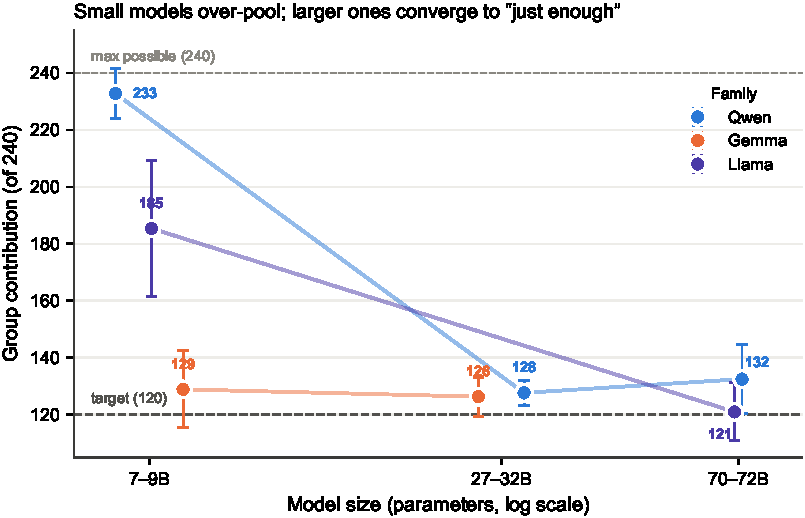
\includegraphics[width=\columnwidth]{fig3_economy_scaling.pdf}
\caption{\textbf{Small models over-pool; larger ones converge to ``just enough''.} Group contribution (of $240$) against model size on a logarithmic axis, connected within family. In every family the largest model pools far less than the smallest, but the decline is not strictly monotonic: Qwen2.5 falls to $127.6$ at 32B and rises again to $132.5$ at 72B. Error bars are standard deviations across games.}
\label{fig:economy}
\end{figure}

\subsection{The one model that fails, fails by language}
Llama-3.1-70B is the only baseline model that did not reach the target reliably, and it is worth being precise about why, because its pooled average is misleading. A mean contribution of $121.0$ appears to place it exactly on the $120$ target, as though it were playing a knife-edge strategy. It is not: that average is a mixture of two well-separated modes. In English it pooled $130.3$ on average, with every game between $124$ and $140$, and reached the target in all thirty games; in Vietnamese it pooled $111.6$, with every game between $108$ and $118$, and reached the target in none. Only five of its sixty games fall anywhere in the interval $115$--$125$. Its $50\%$ reach rate is therefore a language split, not a marginal case, and we return to it in \S\ref{sec:language}.

Because its Vietnamese games always missed the target, this model absorbed $22$ of the $23$ catastrophes suffered in the baseline study; the only other model ever caught was Qwen2.5-32B, once. Conditional on having missed the target, its catastrophe rate was $0.2$, $1.0$ and $1.0$ at $p=0.1$, $0.5$ and $0.9$, against nominal rates of $0.1$, $0.5$ and $0.9$. With only ten independent lottery draws per cell (\S2.6) these realised rates are far too noisy to read as a risk response, which is precisely why we do not treat catastrophe as a dependent variable. The behaviourally meaningful point is that punishment changed nothing: within each language its contribution was flat across risk, so the one model that was repeatedly ruined did not respond by cooperating more.

\subsection{Prompt salience moves the agents far more than risk does}
\label{sec:salience}
If tripling the catastrophe risk barely moves these agents, what does? The A/B arm of the comprehension study answers this directly, and it was run on the same games with the same decoding, so the comparison is internal. Printing the running pool total in the prompt adds no information about incentives: the total is a deterministic function of a history the agent is already shown, and it changes nothing about payoffs, target or risk. It nevertheless moves behaviour by an order of magnitude more than risk does (figure~\ref{fig:salience}). Contributions fell by $95.3$ points for Qwen2.5-7B ($232.5 \to 137.2$, paired $P = 6\times10^{-34}$), by $26.6$ for Llama-3.1-8B ($P = 2\times10^{-17}$), by $8.2$ for Gemma-2-9B ($P = 2\times10^{-6}$) and by $2.9$ for Qwen2.5-32B ($P = 0.003$). The fifth model, Gemma-2-27B, shifted by the same $2.9$ points but not significantly ($P = 0.16$); its target-reach rate nevertheless fell from $100\%$ to $67\%$, because it plays so close to the threshold that a shift too small to detect in contributions is large enough to change the outcome. The two smallest models, which over-contributed most when the total was hidden, are precisely the ones that correct hardest when it is shown.

\begin{figure}[t]
\centering
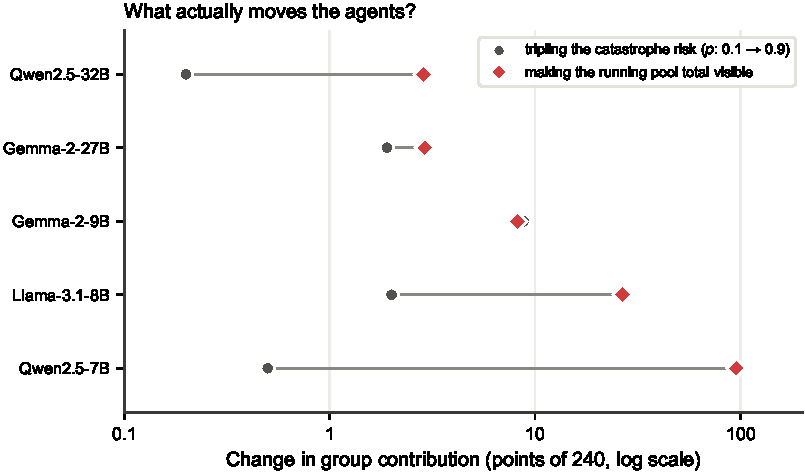
\includegraphics[width=\columnwidth]{fig7_salience.pdf}
\caption{\textbf{Salience beats incentive.} Absolute change in group contribution (of $240$, log axis) produced by two manipulations, for the five models run in both arms: tripling the catastrophe risk from $p=0.1$ to $p=0.9$ (grey circles, paired within seed) versus printing the running pool total in the prompt (red diamonds). The salience manipulation carries no information about payoffs, target or risk, yet dominates for four of the five models.}
\label{fig:salience}
\end{figure}

\subsection{Group composition is a linear engine against a fixed threshold}
\label{sec:composition}
The second manipulation that dwarfs risk is the composition of the group. Replacing cooperative with selfish personas one agent at a time moves contributions monotonically and by a large margin: from all-cooperative to all-selfish, group contribution falls by $100.4$ points for Gemma-2-9B ($148.1\to47.7$, paired $P=6\times10^{-37}$), by $94.0$ for Llama-3.1-8B ($199.4\to105.4$, $P=3\times10^{-24}$) and by $31.8$ for Qwen2.5-7B ($237.7\to205.9$, $P=4\times10^{-28}$). Even the smallest of these is more than three times the largest risk effect anywhere in the study, and the largest is more than ten times it.

What makes this manipulation informative is not only its size but its regularity. Group contribution falls almost perfectly linearly in the number of selfish agents (figure~\ref{fig:composition}(a)), with within-language $R^2$ of $0.95$ for both Gemma-2-9B and Llama-3.1-8B in English and $0.63$--$0.85$ elsewhere. Each model is therefore summarised by two numbers: an intercept, the contribution of an all-cooperative group, and a slope, the cost of converting one cooperative agent into a selfish one. Pooled across languages these are $146.5$ and $-16.6$ for Gemma-2-9B, $199.4$ and $-15.9$ for Llama-3.1-8B, and $234.9$ and $-5.0$ for Qwen2.5-7B.

This two-parameter description explains something that looks, on the raw reach curves, like three qualitatively different failure modes (figure~\ref{fig:composition}(b)). Gemma-2-9B's reach rate collapses immediately, halving at a single selfish agent and reaching zero by five. Llama-3.1-8B holds at or near $100\%$ through four selfish agents and then falls off a cliff, to $52\%$ at five and $28\%$ at six. Qwen2.5-7B never fails at all: it reaches the target in every one of its $420$ composition games, even when all six agents are told to be selfish. Yet all three obey the same linear law. The difference is entirely where each line starts and how steeply it falls relative to a threshold that does not move: Gemma's line crosses $120$ at $1.6$ selfish agents, Llama's at $5.0$, and Qwen's only at $23.0$ - that is, never, since the group has six members. Dramatic differences in apparent robustness are the arithmetic consequence of a linear response meeting a fixed threshold, not evidence of different strategies.

The composition study also delivers the conditions for the decisive risk test of \S\ref{sec:knifeedge}, and it is worth noting what it shows there. In the balanced three-against-three cell, where groups are furthest from any ceiling, reach remains flat in risk for all three models (Llama-3.1-8B and Qwen2.5-7B at $100\%$ at every risk level; Gemma-2-9B at $20\%$, $35\%$ and $25\%$, non-monotonic and within noise), and group contribution varies by less than $2.2$ points across the entire risk range in every model. Making the group's fate genuinely uncertain does not make the agents attend to the probability that decides it.

\begin{figure*}[t]
\centering
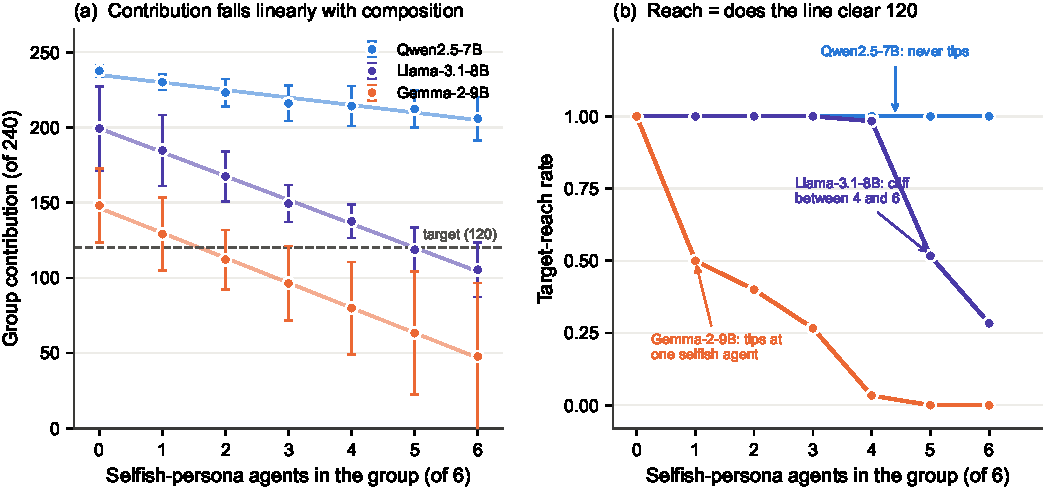
\includegraphics[width=\textwidth]{fig8_composition.pdf}
\caption{\textbf{Group composition is a linear engine against a fixed threshold.} (a)~Group contribution (of $240$) against the number of selfish-persona agents in the six-agent group, for the three open-weight models run in this study; lines are ordinary least-squares fits, points are cell means and error bars are standard deviations across games. The response is close to linear in every model ($R^2$ up to $0.95$ within language). (b)~The corresponding target-reach rates. The three apparently distinct failure modes - immediate collapse, a late cliff, and no failure at all - follow from where each model's line in (a) crosses the fixed target of $120$: at $1.6$, $5.0$ and $23.0$ selfish agents respectively.}
\label{fig:composition}
\end{figure*}

\subsection{A frontier model shows the same pattern, and an extreme language effect}
\label{sec:frontier}
All seven models above are open-weight and share broad training conventions, so we repeated both studies with a frontier API model, GPT-5.4-nano (\S\ref{sec:frontiermethods}). The risk null replicates. In English the model reached the target in all $15$ baseline games at every risk level, pooling $205.6$, $210.8$ and $212.8$ at $p=0.1$, $0.5$ and $0.9$; the paired difference across the full risk range is $+7.2$ points of $240$ ($P=0.025$, $n=5$), again in the right direction and again far too small to change an outcome. In Vietnamese it missed the target in all $15$ games at every risk level, and the risk difference is $-4.4$ points ($P=0.28$), in the wrong direction. In the composition study the same linear engine appears, with $R^2=0.89$ in both languages, an English intercept of $210.5$ and slope of $-18.9$, and a line crossing the target at $4.8$ selfish agents - closely tracking the reach rates of $100\%$ through three selfish agents, $87\%$ at four, $47\%$ at five and $7\%$ at six (figure~\ref{fig:frontier}(b)).

The frontier model's language effect is the largest single effect we measured anywhere. In the baseline study it pooled $209.7$ in English and $62.9$ in Vietnamese, a paired difference of $146.8$ points of $240$ ($P=1\times10^{-16}$, $n=15$), and its target-reach rate went from $100\%$ to $0\%$. This is not a marginal shift in a model living near the threshold, as it was for Llama-3.1-70B: the Vietnamese groups pooled roughly half of the target, and $84$ of the $105$ Vietnamese composition games ended in a realised catastrophe. In Vietnamese the model begins below the threshold even when all six agents are told to be cooperative ($78.7$ of $240$), so the composition line never crosses $120$ at any composition and reach is floored at zero throughout (figure~\ref{fig:frontier}(b)) - the mirror image of the ceiling censoring that limits the English cells.

Placed on a common axis (figure~\ref{fig:frontier}(c)), the manipulations separate by orders of magnitude for this model: catastrophe risk moves group contribution by $4.4$--$7.2$ points, group composition by $65.1$--$112.4$, and language by $146.8$. The one manipulation the game says should matter is the smallest of the four by a factor of nine to thirty-three.

\begin{figure*}[t]
\centering
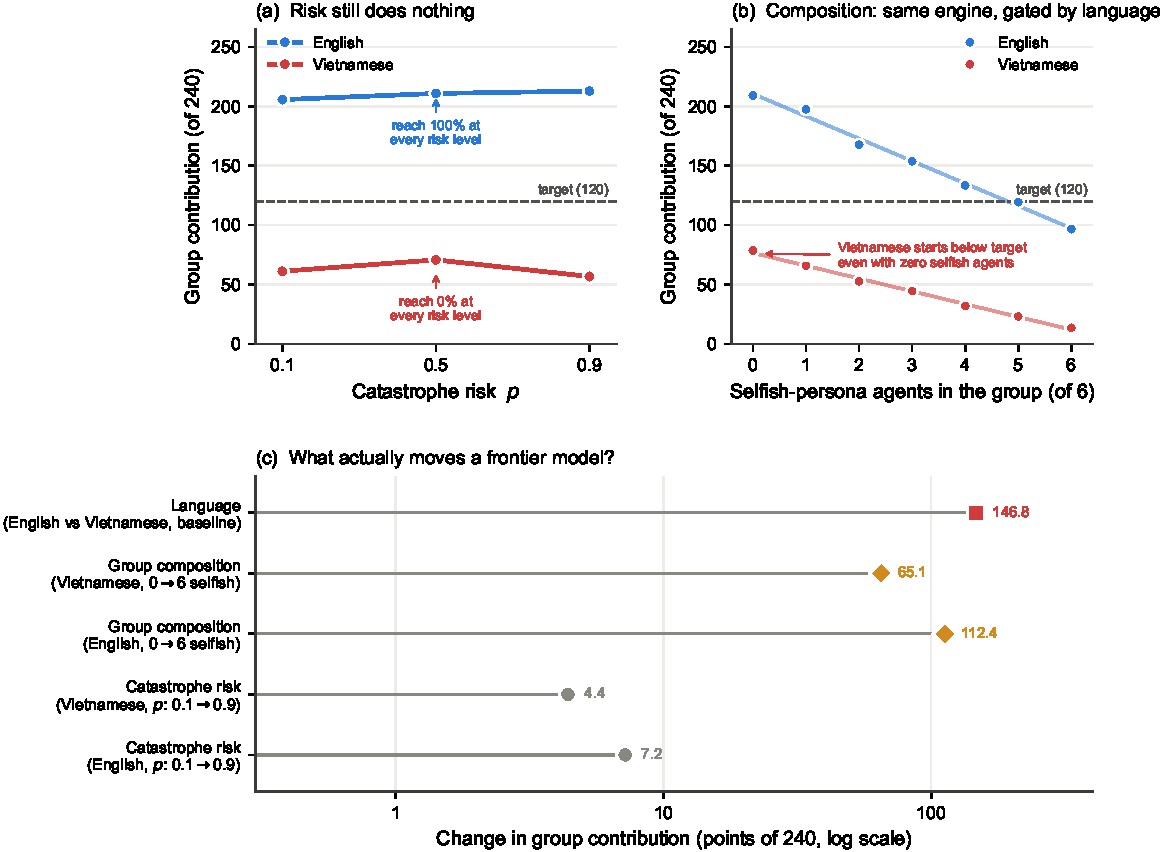
\includegraphics[width=\textwidth]{fig9_frontier.pdf}
\caption{\textbf{A frontier model reproduces the pattern.} GPT-5.4-nano, $30$ baseline and $210$ composition games. (a)~Group contribution against catastrophe risk, by language: flat in both, with English reaching the target in $100\%$ of games at every risk level and Vietnamese in $0\%$. (b)~The composition study shows the same near-linear engine as the open-weight models ($R^2=0.89$ in both languages), but the Vietnamese line starts below the target even with zero selfish agents, so it never crosses. (c)~The four manipulations on a common logarithmic axis. Risk is the smallest by a factor of nine to thirty-three.}
\label{fig:frontier}
\end{figure*}

\subsection{What the agents can and cannot do}
The behavioural deviation might, in principle, be a failure of comprehension: perhaps the models over-cooperated and ignored the risk because they did not grasp the rules or could not read the game. The in-situ probes rule this out. Accuracy on the \emph{Rules} axis was uniformly high, from $93.8\%$ for Llama-3.1-8B to $100\%$ for the five largest models, and accuracy on the \emph{Time} axis - reading specific events from the history - ranged from $82\%$ to $99\%$ (figure~\ref{fig:comprehension}). One probe asked the model to state the catastrophe probability of the game it was playing, and every model answered almost always correctly: $98.1\%$ for Qwen2.5-7B, $91.4\%$ for Llama-3.1-8B and $100\%$ for the other five (figure~\ref{fig:mechanism}(b), upper curve). We are deliberately modest about what this shows. The decision prompt prints the catastrophe probability verbatim, so the probe is a retrieval task, and these models copy printed values at ceiling throughout our data. It establishes that the risk was legible in the context the agent decided from - which is worth establishing, since it rules out the possibility that the number was lost or garbled - but it does not show that the agent represented the risk as a decision-relevant quantity, and it cannot distinguish an agent that weighed the risk and set it aside from one that never entered it into a calculation at all.

\begin{figure}[t]
\centering
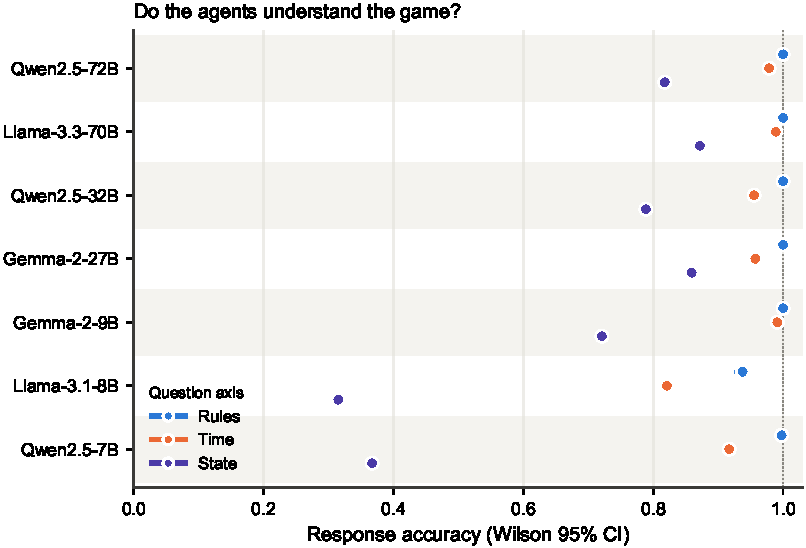
\includegraphics[width=\columnwidth]{fig4_comprehension_category.pdf}
\caption{\textbf{Comprehension by question axis.} Response accuracy (dots) with Wilson $95\%$ confidence intervals for each model, ordered by size (smallest at the bottom), on the Rules, Time and State axes; alternating bands group the three dots belonging to one model, and with $2{,}880$--$28{,}200$ probes per point the intervals are narrower than the markers. Rules is at ceiling and Time is high ($82$--$99\%$) for all models; State (cumulative situation) is the only axis that varies widely, and it improves broadly with scale.}
\label{fig:comprehension}
\end{figure}

\subsection{Reading is not adding, and adding scales}
The only comprehension axis on which the models struggled was \emph{State}, the current cumulative situation, and the reason is specific and revealing. When we asked for a quantity that was printed verbatim in the prompt - for example, a player's own remaining money - accuracy was high for every model: under the same hidden-pool prompt used for the comparison below, five of the seven answered at or within a fraction of a point of ceiling, and Qwen2.5-7B scored $89.0\%$. The exception is Llama-3.1-8B, at $68.8\%$ overall and only $46.0\%$ in English: that model cannot reliably read the printed value either, so it is a poor test of the dissociation, and the contrast below should be read from the other six. When we asked for the same kind of quantity that had to be \emph{summed} across rounds, namely the running pool total while it was hidden from the prompt, small models collapsed: Qwen2.5-7B answered correctly only $14.3\%$ of the time and Llama-3.1-8B only $9.8\%$, even though both could read a printed value almost perfectly (figure~\ref{fig:mechanism}(a)). That the failure is arithmetic rather than perceptual is confirmed by the A/B manipulation: when the same pool total was printed rather than hidden, accuracy jumped to $92$--$100\%$ across the board. Reading, in other words, is not adding.

This cumulative-addition deficit is a property of small models that scale largely removes. Accuracy on the hidden pool total rose steeply, if not perfectly monotonically, with size: $14.3\%$ and $9.8\%$ for the 7B and 8B models, $21.2\%$, $61.5\%$ and $43.5\%$ for the 9B, 27B and 32B models, and $81.7\%$ and $88.2\%$ for the 70B and 72B models (figure~\ref{fig:mechanism}(b), lower curve); the two local reversals fall between families rather than within them. The juxtaposition in figure~\ref{fig:mechanism}(b) is central to the paper: knowledge of the risk is flat and near-perfect across the whole size range, while the ability to track cumulative state climbs steeply with scale. By 70--72B the models both know the risk and can add the pool - and they still ignore the risk.

\begin{figure*}[t]
\centering
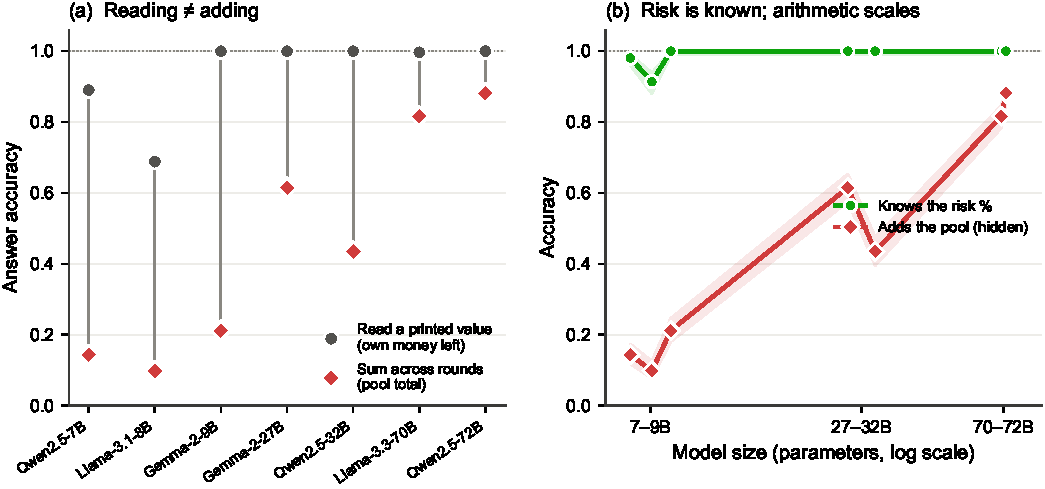
\includegraphics[width=\textwidth]{fig5_mechanism.pdf}
\caption{\textbf{The gap is arithmetic, and it closes with scale.} (a)~Under the default hidden-pool prompt, accuracy on a value the agent can read straight off the prompt (its own money left, grey circles) versus a value it must sum across rounds (the pool total, red diamonds). Small models can read but cannot add. The same-question control is the A/B in the text: printing the pool total lifts accuracy on that identical question to $92$--$100\%$. (b)~Knowledge of the catastrophe probability (green) is flat and near-perfect across the size range, whereas the ability to sum the hidden pool (red) rises steeply with scale. Even where both are near-ceiling, behaviour remains risk-insensitive. Bands are Wilson $95\%$ intervals.}
\label{fig:mechanism}
\end{figure*}

\subsection{Language preserves knowledge but degrades arithmetic}
\label{sec:language}
Running every condition in English and Vietnamese revealed a clean dissociation (figure~\ref{fig:language}). Behaviourally, the two languages produced identical target-reach rates for five of the seven open-weight models. Qwen2.5-32B dipped slightly ($100\%$ in English versus $93.3\%$ in Vietnamese, and its single catastrophe fell in Vietnamese), and Llama-3.1-70B collapsed outright, from $100\%$ in English to $0\%$ in Vietnamese, so that its overall $50\%$ was entirely a language split rather than a risk effect. In comprehension, language left rule and risk knowledge essentially untouched - Rules accuracy differed by under one percentage point between languages and the risk probability was read correctly in both - but it selectively attacked the arithmetic. State accuracy fell from $73.6\%$ in English to $61.8\%$ in Vietnamese, an almost twelve-point drop. The damage was concentrated in the middle of the range rather than at the bottom: Gemma-2-9B lost the most ($87.8\%$ to $56.4\%$, $31.5$ points), whereas the two models that were already worst at cumulative addition had the least left to lose (Qwen2.5-7B $13.6$ points, Llama-3.1-8B $11.3$ points), and Llama-3.3-70B was unaffected (Vietnamese in fact $0.8$ points higher). Language, then, changes what the models can compute far more than what they know.

The frontier model turns this from a tail risk into the dominant effect. Its $146.8$-point language gap (\S\ref{sec:frontier}) is larger than any other effect in the study, and it converts a model that never fails into one that never succeeds. Two of our nine model-language pairings therefore invert their outcome entirely on a change of language that leaves the game, the payoffs and the stated risk identical.

\begin{figure*}[t]
\centering
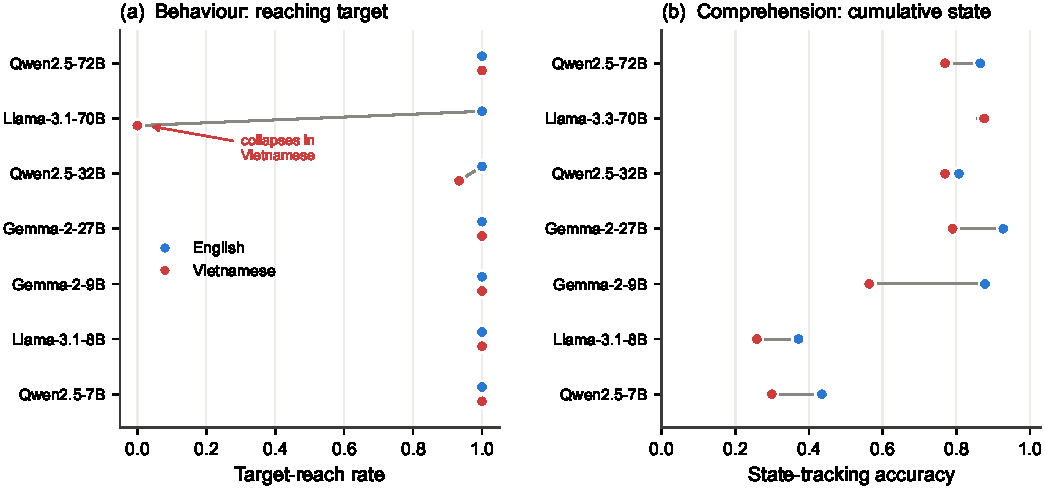
\includegraphics[width=\textwidth]{fig6_language.pdf}
\caption{\textbf{English versus Vietnamese.} (a)~Target-reach rate in each language for the seven open-weight models, the two points of a pair offset vertically so that coincident values stay visible. Behaviour is identical across languages for five of the seven; Qwen2.5-32B dips slightly ($100\%$ to $93.3\%$) and Llama-3.1-70B collapses from $100\%$ to $0\%$ in Vietnamese. (b)~Cumulative-state accuracy in each language. Vietnamese selectively degrades the arithmetic; the largest loss is Gemma-2-9B ($31.5$ points), while the weakest adders have least left to lose and Llama-3.3-70B is unaffected.}
\label{fig:language}
\end{figure*}

\begin{table*}[t]
\centering
\caption{\textbf{Headline results per model.} Behavioural quantities pooled over risk and language ($60$ games/model for the open-weight panel, $30$ for the frontier model): target-reach rate, group contribution (of $240$) and realised catastrophe rate. Comprehension quantities from the in-situ probes: accuracy at stating the catastrophe probability (\emph{risk knowledge}) and at summing the hidden pool (\emph{cumulative arithmetic}). Comprehension used the Llama-3.3 revision at 70B, and was not run for the frontier model. The composition column gives the change in group contribution from an all-cooperative to an all-selfish group, for the four models run in that study. Human target-reach rates rise from $0\%$ to $50\%$ with risk.}
\label{tab:headline}
\begin{tabular}{@{}lcccccccc@{}}
\toprule
& & \multicolumn{3}{c}{Behaviour} & Composition & & \multicolumn{2}{c}{Comprehension} \\
\cmidrule(lr){3-5}\cmidrule(lr){8-9}
Model & Size & Reach & Contribution & Catastrophe & $\Delta$ 0$\to$6 selfish & & Risk knowledge & Cumulative arithmetic \\
\midrule
Qwen2.5-7B    & 7B  & $100\%$  & $232.7$ & $0\%$   & $-31.8$  & & $98.1\%$ & $14.3\%$ \\
Llama-3.1-8B  & 8B  & $100\%$  & $185.4$ & $0\%$   & $-94.0$  & & $91.4\%$ & $9.8\%$  \\
Gemma-2-9B    & 9B  & $100\%$  & $128.9$ & $0\%$   & $-100.4$ & & $100\%$  & $21.2\%$ \\
Gemma-2-27B   & 27B & $100\%$  & $126.3$ & $0\%$   & --       & & $100\%$  & $61.5\%$ \\
Qwen2.5-32B   & 32B & $96.7\%$ & $127.6$ & $1.7\%$ & --       & & $100\%$  & $43.5\%$ \\
Llama-3.1-70B & 70B & $50\%$   & $121.0$ & $36.7\%$& --       & & $100\%$\textsuperscript{*} & $81.7\%$\textsuperscript{*} \\
Qwen2.5-72B   & 72B & $100\%$  & $132.5$ & $0\%$   & --       & & $100\%$  & $88.2\%$ \\
\midrule
GPT-5.4-nano  & --  & $50\%$\textsuperscript{\dag}   & $136.3$\textsuperscript{\dag} & $40\%$\textsuperscript{\dag} & $-112.4$\textsuperscript{\ddag} & & -- & -- \\
\bottomrule
\end{tabular}\\[2pt]
{\footnotesize \textsuperscript{*}Llama-3.3-70B in the comprehension study.
\textsuperscript{\dag}Pooled over language; the pooled figure is a mixture of $100\%$ reach in English and $0\%$ in Vietnamese and should not be read as a knife-edge strategy (\S\ref{sec:frontier}).
\textsuperscript{\ddag}English; the Vietnamese figure is $-65.1$ from a starting point already below the target.}
\end{table*}

\section{Discussion}

The central result of this study is a comparison of manipulations measured under one game. Humans in this dilemma cooperate more when the catastrophe is more likely. Across an order of magnitude of open-weight scale and one frontier model, none did so to any consequential degree - and, critically, the null holds where it can be tested cleanly. In the conditions where roughly half of the groups succeed and half fail, so that the outcome variable is free and the catastrophe is a live possibility, a ninefold increase in the probability of ruin moves contributions by $+0.97$ of $240$ in the open-weight panel and $+7.5$ in the frontier model, neither distinguishable from zero. Against that, three manipulations that carry no information about payoffs, target or risk each move the same quantity by tens to over a hundred points: displaying a number the agent already had the information to compute, changing which dispositions are named in the six prompts, and changing the language those prompts are written in.

The unifying observation is that all three of the manipulations that work are delivered through the prompt, and the one that does not work is delivered through the incentive structure. This is a sharper statement than ``LLMs are risk-insensitive'', and it has a different implication. It is not that these agents fail to respond to their situation - they respond vigorously, and in the normatively sensible direction, to being told who they are and to being shown the state of play. It is that the channel through which a game communicates stakes, namely the consequences attached to outcomes, is the channel they attend to least. An agent that adjusts its contribution by a hundred points when a neighbouring prompt says ``selfish'', and by one point when its own probability of losing everything rises from one-in-ten to nine-in-ten, is not weighing costs and benefits in any recognisable sense.

The composition study adds a second lesson, about how such systems fail. The response to composition is close to linear, and the threshold is fixed, so whether a group succeeds is determined by where a straight line crosses a horizontal one. This makes collective failure both highly predictable and highly discontinuous: two models with similar per-agent behaviour can have completely different tipping points, and a model can appear perfectly robust across a wide range of compositions and then fail almost completely within one further step. Qwen2.5-7B never failed in $420$ composition games not because it resists selfish framing better than the others - its slope is shallower, but it is genuinely negative - but because its intercept is so high that six selfish agents are not enough to bring it down. Robustness, here, is a property of the margin between an intercept and a threshold, not of anything one would call resilience. For anyone deploying a fleet of agents to a shared quantitative goal, the practical implication is that the observable per-agent quantities are the intercept and slope, and that these, not the observed success rate, are what determine how much adverse composition the system can absorb.

We are careful about what the comprehension gate does and does not establish. The battery tests whether a model can report the rules, read the history and sum the state; it does not test whether the model can put $p$ to work decision-theoretically - no question asks for the expected payoff of missing the target at this $p$, or which contribution maximises it. Our results therefore rule out the explanation that the models misread the game, but they do not distinguish a model that has weighed the risk and set it aside from one that recalls the number without ever entering it into a calculation. Both are dispositions rather than misunderstandings, and the distinction between them is the natural target of a follow-up study. A second caveat is one of coverage: the comprehension panel used Llama-3.3-70B where the behavioural panel used Llama-3.1-70B, so the single open-weight model with genuine behavioural variance has no comprehension data of its own, and the joint claim rests principally on Qwen2.5-72B, with Gemma-2-27B and Qwen2.5-32B at the middle of the range. The frontier arm has no comprehension data at all.

If the agents are not tracking risk, what are they tracking? The evidence points to the contents of the prompt. Our own prompt names the equal-split solution, and the models that converge on ``just enough'' converge on very nearly that number, with Gemma-2-9B in English reproducing it exactly in all thirty games. Adding one more number to the prompt - the running total - moves them again, and by much more; adding one sentence about disposition moves them further still. A parsimonious reading of the whole panel is that these agents are executing the most salient available instruction rather than solving a dilemma, and that their apparent cooperativeness is in part an artefact of what we told them. A second contributing factor is plausible but, on our data, unproven: instruction tuning. Every model we studied was fine-tuned to be helpful and harmless~\cite{ouyang2022instructgpt,bai2022hhrlhf}; those procedures optimise for helpfulness and harmlessness rather than for cooperation as such, and we can only conjecture - not demonstrate here - that the resulting disposition generalises into a bias toward reaching a shared goal. Our data are at least consistent with such a tendency overriding the incentive structure of the game: the models converge on ``reach the target'' as a default and calibrate only how much private surplus to keep, not whether the target is worth reaching given the risk. This reading is reinforced by what scale does and does not change. Scaling from 7B to 72B improves a genuinely cognitive sub-skill, cumulative arithmetic, from near-chance to near-ceiling, exactly the kind of capability that larger models are known to acquire~\cite{wei2022emergent}; yet the same scaling leaves the behavioural prior untouched, and the frontier model shows the same prior again. Capability and the disposition to act on incentives are, here, decoupled - a caution for the assumption that more capable agents will automatically behave more like rational, risk-responsive decision-makers.

These findings connect to prior work whose picture is more mixed than a single summary allows. Some studies report LLMs that are markedly more cooperative and more forgiving than humans in repeated dilemmas~\cite{fontana2024nicer,phelps2023investigating}; others report the opposite temperament, with GPT-4 retaliating unforgivingly after a single defection~\cite{akata2023playing}, and most models failing to sustain a shared resource without explicit institutional scaffolding~\cite{piatti2024cooperate}. Our result sits with the first group and sharpens it: in a dilemma structured by risk rather than by a payoff matrix, over-cooperation appears as an insensitivity to the very quantity that should govern it. The composition result also bears on the practice of persona-conditioning LLMs to stand in for heterogeneous human populations~\cite{argyle2023out,aher2023using}: personas do move behaviour substantially and monotonically, which is encouraging for that practice, but in our data they move it far more reliably than the game's own incentives do, which means a persona-conditioned population may reproduce the distribution of stated dispositions while badly misrepresenting how that population would respond to changing stakes. Methodologically, the study extends the in-situ understanding-check paradigm from the two-player prisoner's dilemma~\cite{fontana2024nicer} to an $N$-player threshold game and shows that a single, well-chosen probe - can the model state the risk it faces? - separates one important confound, misreading, from a behavioural claim. We suggest that behavioural evaluations of LLM agents should routinely include such gates, and that null results on an incentive manipulation should routinely be accompanied by an uncensored subset in which the null can actually be tested.

Our results carry four practical implications. First, LLM agents are unreliable surrogates for humans in risk-structured collective decisions: they fail to reproduce the human risk response, and would, for example, predict near-certain cooperation at a level of risk where human groups in fact reach the target only half the time. (The comparison is not uniformly unflattering: at $p=0.9$ the least ceiling-bound open-weight model, Llama-3.1-70B, reaches the target in exactly half of its games, as human groups do; the divergence is concentrated at low risk, where the agents cooperate and humans do not.) Second, because the behavioural prior is invariant to scale while the underlying numeracy is not, one cannot infer an agent's incentive-responsiveness from its competence; more capable agents in a fleet may be quieter about, not freer of, a shared disposition. Third, group composition is both the most reliable lever and the most treacherous one: it moves behaviour linearly and predictably, but converts into success or failure through a threshold, so systems can look robust right up until they are not. Fourth, language is not neutral: deploying the same model in a lower-resource language preserved its factual knowledge of the game but degraded its quantitative reasoning and, for two of our models, inverted their outcomes entirely. Multilingual deployment can therefore silently move quantitative behaviour even where surface comprehension looks intact.

\label{sec:limits}
Several limitations bound these conclusions, and the first is severe enough that we place it ahead of the others. Our decision prompt names the equal-split solution. An agent that contributes 2 is therefore consistent with a cooperative disposition, with plain instruction-following, or with anchoring on the only number the prompt offers, and this study cannot tell them apart. The evidence that this is not hypothetical is in our own data: Gemma-2-9B produced a group total of exactly $120.0$ in all thirty English games, with zero variance, and Gemma-2-27B did the same in Vietnamese. Any claim in this paper about cooperative dispositions should be read as a claim about behaviour under a prompt that supplies a focal action; the clean experiment removes the hint and re-runs, and we regard that as the necessary sequel rather than an optional extension. For the same reason we have framed our central results as comparisons between manipulations measured under the identical prompt, since those contrasts are internal and survive the confound.

The remaining limitations are of coverage and implementation. The composition study covers only the three smallest open-weight models and the frontier model, so the linear-engine description is established at 7--9B and at one frontier model, not across the full size range; whether the larger open-weight models obey the same law is untested. The frontier arm is a single model at five repetitions, served through an interface that does not honour per-turn seeds, so its games are unpaired and its confidence intervals correspondingly wide - the $+7.5$-point risk estimate there is a null by virtue of its interval, not by virtue of precision. Its Vietnamese cells are floored rather than ceilinged, which limits what they can show for the same reason the English ceiling limits the baseline. The persona-to-seat permutation is deterministic rather than uniformly random and is not perfectly balanced across seats, so we make no claims about position effects. The groups were homogeneous in model and mute: all six agents were the same model and could not communicate, whereas human cooperation is shaped by heterogeneity and cheap talk, so our estimates speak to a specific, controlled regime rather than to open multi-agent interaction. The catastrophe was a single end-of-game lottery drawn from a schedule shared across conditions, which makes realised disaster rates uninformative and is why we treated reach rate and contribution as the primary dependent variables. Two confounds bound the scaling claim in particular. The 70B and 72B models were served with activation-aware weight quantisation while the smaller models were not, so ``scale'' is not a perfectly clean manipulation; and the Milinski design is old and widely reproduced, so it is likely present in every model's training corpus, meaning an agent may partly be recognising a familiar task rather than reasoning about it afresh. We studied instruction-tuned models only, so the prior we describe is a property of models as deployed and may differ for base models; without base-model controls the attribution to instruction tuning remains a conjecture. Finally, we examined a single dilemma; whether the same disposition governs other risk-structured games, and whether it can be moved by targeted prompting or fine-tuning, are open questions.

Those questions define the natural next steps, and one of them we can already answer. We had expected that forcing explicit accounting - printing the running total each round - would repair the small models' arithmetic without touching their behaviour, on the reasoning that the risk they must respond to is not the state they must add. That expectation was wrong, and informatively so: printing the total changed contributions more than any incentive manipulation in the study. The remaining steps are to remove the equal-split hint and re-run; to extend the composition sweep across the full size range, which would test whether the intercept-and-slope description is general; to compare base and instruction-tuned checkpoints, without which the attribution to instruction tuning stays a conjecture; and to introduce heterogeneous groups and communication, which would test whether anything here survives social pressure.

\section{Conclusion}

Eight instruction-tuned language models - seven open-weight models from 7 to 72 billion parameters across three families, and one frontier model - played a replication of the collective-risk social dilemma. None reproduced the human response to risk. The null is not an artefact of a ceiling: in the conditions where roughly half of groups succeed and half fail, and the catastrophe is therefore a live possibility, raising the probability of ruin ninefold moves group contribution by $+0.97$ of a possible $240$ ($P=0.54$) in the open-weight panel and by $+7.5$ ($P=0.26$) in the frontier model. Against that null, three manipulations that carry no incentive information at all move the same quantity by one to two orders of magnitude more: printing the running pool total (up to $95.3$ points), changing the prosocial composition of the group ($31.8$--$112.4$ points), and switching the prompt language ($146.8$ points, inverting a $100\%$ reach rate to $0\%$). The composition effect is close to linear in the number of selfish agents, so collective success is decided by where a straight line crosses a fixed threshold - which is why models with similar behaviour fail at completely different compositions, and why apparent robustness can vanish in a single step. Comprehension probes bound the explanation: the agents recite the rules and read printed quantities at ceiling, while cumulative summation is a small-model gap that closes with scale; but they cannot establish that risk was ever treated as a decision variable, since the prompt prints it. Our own prompt also names the equal-split solution, and some models reproduce it exactly, so we cannot separate cooperative disposition from compliance with a supplied focal point. The methodological conclusion is the robust one: before a behavioural regularity in LLM agents is attributed to a preference, it should be tested against prompt-side controls that change what the agent is shown without changing what the game makes costly - and any null on an incentive manipulation should be reported alongside a subset of conditions in which that null could have been falsified.

\enlargethispage{20pt}

\ethics{}

\dataccess{}

\aucontribute{}

\competing{}

\funding{}

\ack{}

\bibliography{refs}

\end{document}
